\chapter{Hawking radiation as seen by Observers}
\label{sec:bh}
\section{The metric}
In this thesis we will only use the Schwarzschild-metric to describe stars and black holes (which means that they have no charge and no angular momentum). The metric for an spherical symmetric object with mass \(M\) is given by
\begin{align}
\dd s^2 &= -f(r)\dd{t^2} + \frac{1}{f(r)}\dd{r^2} + r^2 \dd{\Omega} &\dd{\Omega} = \dd{\theta^2} + \sin[2](\theta) \dd{\varphi^2} 
\end{align}
where \(f(r) = 1-\frac{2M}{r}\). The metric is only valid outside the boundary of the star or for \(r > 2M\). The two vector fields \(\partial_t\) and \(\partial_\varphi\) are killing.

\section{The Klein-Gordon-Equation in the Schwarzschild metric}

Consider a static spherical star where the outer metric is the Schwarzschild metric (i.e. non rotating and uncharged). It's important that we are considering a star because a black hole does not provide a global timelike killing vector field (analytic extension of \(\partial_t\) leads to a spacelike vectorfield inside the black hole). From now on we will only consider the outer region. To achieve a global solution one need to match inner with outer solutions.

The Klein-Gordon-Equation \(\nabla_\mu\nabla^\mu \phi = 0\) can be written as:
\begin{align}
-\frac{r^2}{f(r)}\partial_t^2 \phi + \qty(\partial_r r^2 f(r) \partial_r) \phi - L^2 \phi = 0
\end{align}

where \(L^2\) is the usual angular momentum operator.

\subsection{Spherical Modes}

Since the spacetime is spherical symmetric and has the killing vector field \(\partial_t\) we can do the following ansatz for the modes
\begin{align}
u_{\omega l m} = A e^{-i\omega t} \frac{R_{\omega l}}{r}Y_l^m (\theta, \varphi)
\end{align}

Plugging this into the Klein-Gordon-Equation \(\nabla_\mu\nabla^\mu u_{\omega l m} = 0\) yields to the following equation for \(R_{\omega l}\) (see for example \cite{davies}):
\begin{align}
\dv[2]{R_{\omega l}}{r_*} + \omega^2 R_{\omega l} -\qty(\frac{l(l+1)}{r^2} + \frac{f'(r)}{r})f(r) R_{\omega l} &= 0\\
\dv[2]{R_{\omega l}}{r_*} + \omega^2 R_{\omega l} - \order{r^{-2}} R_{\omega l} &= 0
\end{align}

So for \(\omega r \gg l\) one can neglect the \(r\) dependent part. In this case we find the asymptotic solutions
\begin{align}
R_{\omega l} &= e^{\pm i \omega r_*}\\
u_{\omega l m} &=  \frac{A_{\omega l m}}{r} e^{-i\omega t + i\omega r_*} Y_l^m (\theta, \varphi) + \frac{B_{\omega l m}}{r} e^{-i\omega t - i\omega r_*} Y_l^m (\theta, \varphi)\\
	&= \frac{A_{\omega l m}}{r} e^{-i\omega u} Y_l^m (\theta, \varphi) + \frac{B_{\omega l m}}{r} e^{-i\omega v} Y_l^m (\theta, \varphi)
\end{align}

Unfortunately we either cannot determine the (quite important) phase between \(A_{\omega l m}\) and \(B_{\omega l m}\) nor can we normalise the modes by integrating over all space. Instead I will impose that very far away from the star (where \(r_* \approx r\)) the field behaves as in Minkowskispace (which means that e.g. experiments give the same results). This implies that \(D^+(\vb{x},\vb{x}')\) is the same as in Minkowskispace. Comparing with the asymptotic spherical modes in Minkowskispace (see eq. \eqref{equ:bessel_asympt}) yields to:
\begin{align}
u_{\omega l m} &=  \frac{1}{\sqrt{\pi\omega}} e^{-i\omega t} \frac{\sin(\omega r_* - l\frac{\pi}{2})}{r} Y_l^m (\theta, \varphi)  = \frac{r_*}{r} u_{\omega l m}\upd{M}(r_*,\theta,\varphi)\\
&= \frac{i^{-l}}{2i\sqrt{\pi\omega}r} e^{-i\omega u} Y_l^m (\theta, \varphi) - \frac{i^{l}}{2i\sqrt{\pi\omega}r} e^{-i\omega v} Y_l^m (\theta, \varphi)
\label{equ:bh_modes}
\end{align}

\subsection{The Wightman function}
The next step would be to calculate the Wightman function \(D^+(\vb{x}, \vb{x}')\). Note that since \(\partial_t\) is a timelike killing vector we define the ground state \(\ket*{0}\) by \(a_{\omega l m} \ket*{0} = 0\) and use eq. \ref{equ:wightman_modes}.
\begin{align}
D^+(\vb{x}, \vb{x}') = \int_0^\infty \frac{\dd{\omega}}{\pi\omega} \sum_{l,m} e^{-i\omega(t-t')} \frac{\sin(\omega r_* - l\frac{\pi}{2})}{r} \frac{\sin(\omega r_*' - l\frac{\pi}{2})}{r'} Y_l^m(\theta,\varphi) Y_l^{m*}(\theta',\varphi')
\end{align}

Since this integral is nearly the same as in Minkowskispace (see eq. \ref{equ:wightman_minkoski_spherical}) we also encounter the same problems, namely the IR divergence and the fact that it is non-zero only in two directions. This is due to the fact that the approximation \(\omega r \gg l\) breaks down for small \(\omega\) and for large \(l\). Recall that the problems in the non approximate calculation in Minkowskispace didn't occur because the \(j_l(\omega r)\) remain finite at \(\omega \to 0\). In other words the essential feature of the \(j_l(\omega r)\) is that they let all the \(\cos(\omega ...)\) terms in the integral drop to zero for \(\omega \to 0\) instead of \(\cos{0} = 1\) in the approximate case. Therefore we can assume that the same happens for exact solutions around the star.

Unfortunately the exact behaviour for small \(\omega\) is the same as for small \(r\) which will depend on the specific geometry of the star. But the metric of a star is almost flat (since the radius of a star \(R_0\) is much bigger than its Schwarzschildradius \(R_S\)). Therefore we will approximate the global mode by replacing the sine with the spherical Bessel function:
\begin{align}
u_{\omega l m} &= \frac{\sqrt{\omega}}{\sqrt{\pi}} e^{-i\omega t} \frac{r_*}{r} F(r) j_l(\omega r_*) Y_l^m (\theta, \phi) = \frac{r_*}{r} F(r) u_{\omega l m}\upd{M}(r_*,\theta,\phi)
\end{align}

We introduced an extra factor \(F(r)\) to correct the \(r\) dependence again. This factor must approach \(1\) at infinity. Because the modes now are the same (up to a prefactor and replacing \(r \to r_*\)) as in Minkowski space we can find the Wightman function by adjusting the Wightman function of Minkowski space (see eq. \eqref{equ:qft_inertial})
\begin{align}
D^+(\vb{x}, \vb{x}') &= -\frac{1}{4\pi^2}\frac{r_* r_*' F(r) F(r')}{r r'} \frac{1}{(t-t'-i\varepsilon)^2 - |\va{x}_*-\va{x}_*'|^2}\\
	&=  -\frac{1}{4\pi^2}\frac{r_* r_*' F(r) F(r')}{r r'} \frac{1}{(t-t'-i\varepsilon)^2 - r_*^2 - r_*'^2 + 2r_*r_*' \cos{\alpha}}
\end{align}

where \(\va{x}_*\) is obtained by replacing \(r \to r_*\) in \(\va{x}\) and \(\alpha\) is the angle between the two vectors. We still have the factor \(F(r)\). This can be fixed because we know the behaviour around \(\vb{x} \approx \vb{x}'\) by eq. \eqref{equ:static_normal}. First we know exact that for \(\va{x} = \va{x}'\) it should look like \(-\frac{1}{4\pi^2}\frac{1}{f(r) (t-t')^2}\). This implies \(F(r) = \frac{r}{r_* \sqrt{f(r)}}\). Second for \(t = t'\) the denominator is given by the spatial distance \(|\va{x} - \va{x}'|^2\). The distance between two infinitesimal separated \(r\) and \(r + \dd{r}\) is given by \(|\va{x}(r+\dd{r}) - \va{x}(r)| = \sqrt{g_{rr}} \dd{r} = \frac{\dd{r}}{\sqrt{f(r)}}\). But \(|r_*(r+\dd{r}) - r_*(r)| = \dv{r_*}{r} \dd{r}= \frac{\dd{r}}{f(r)}\). Again we can correct this by setting \(F(r) = \frac{r}{r_* \sqrt{f(r)}}\). Since both independent arguments lead to the same result we conclude that the asymptotic form of the Wightmanfunction is given by:
\begin{align}
D^+(\vb{x}, \vb{x}') &= -\frac{1}{4\pi^2 \sqrt{f(r)f(r')}} \frac{1}{(t-t'-i\varepsilon)^2 - |\va{x}_*-\va{x}_*'|^2}\\
	&=  -\frac{1}{4\pi^2 \sqrt{f(r)f(r')}} \frac{1}{(t-t'-i\varepsilon)^2 - r_*^2 - r_*'^2 + 2r_*r_*' \cos{\alpha}}
\end{align}

\subsection{The Wightman function after the collapse}
To calculate the Wightman function after the collapse we will apply the result of Hawking to find that the expectation value of two operators thereafter is given by the thermal expectation value with \(\beta = 8\pi M\) in the spacetime before the collapse. The corresponding temperature \(T_H = \frac{1}{8\pi M k\ind{B}}\) is called Hawking temperature. \cite{hawking}

Therefore the (vacuum) Wightman function at late times is given by the thermal Wightman function at early times (it can be computed analogously to the one in Minkowski space)
\begin{align}
D^+_\beta(\vb{x},\vb{x}') &= -\frac{1}{4\beta^2\sqrt{f(r)f(r')}} \frac{1}{\sinh[2](\frac{\pi}{\beta}\sqrt{(t-t')^2 - |\va{x}_*-\va{x}_*'|^2})}
\label{equ:bh_wightman_thermal}
\end{align} 

\section{Observers in the Schwarzschildmetric}

In this section we will finally calculate what an observer will see when moving on static, circular and radial trajectories using the thermal Wightman function. We are not interested in the concrete spectrum but rather in the observed temperature. Apart from the static trajectories we cannot solve this analytically, so we need to use numerical methods (see section \ref{sec:app_num}). For a static and circular observer we will also calculate the observed spectrum in the spacetime before the collapse (using the vacuum Wightman function) because we dealt with that before in section \ref{sec:static_observers}.

\subsection{Static observer}
\subsubsection{Before the collapse}
We already know by lemma \ref{lemma:static_static} that a static observer will not see any excitations. We will now show that this is also true when using our approximate form of \(D^+\). A static observer is given by \(t = \frac{\tau}{\sqrt{f(r)}}\) and all other coordinates constant. Inserting this into the Wightman function yields
\begin{align}
D^+(\vb{x}(\tau), \vb{x}(\tau')) =  -\frac{1}{4\pi^2} \frac{1}{(\tau-\tau'-i\varepsilon)^2}
\end{align} 

This is the same as for an inertial observer in Minkowski space (see eq. \ref{equ:qft_inertial}). So a static observer indeed does not recognize any particles.

\subsubsection{After the collapse}

The thermal Wightman function is given by
\begin{align}
D^+_\beta(\vb{x}(\tau),0) &= -\frac{1}{4\beta^2f(r)} \frac{1}{\sinh[2](\frac{\pi}{\beta\sqrt{f(r)}} \tau)}
\end{align}

which results in an observed temperature of \(T = f(r)^{-1/2} T\ind{H}\) which agrees with the Tolman effect found in section \ref{sec:static_observers_thermal}. So a static observer will see a slightly higher temperature than the Hawking temperature.

Since we know the exact result we can use this as a benchmark for our method to approximate the temperature. Running this on a static observer \todo{ok?} gives the result depicted in fig. \ref{fig:bh_stat}. It fits with the Tolman relation over all orders of magnitude\todo{genauer?}. The small difference lies within the numerical errors\footnote{Note that all error depicted in the errorbars is the estimated numerical error, not errors induced by the approximative Wightman function}. We can therefore conclude that our method is suitable for determining the temperature. 

\begin{figure}[h]
  \centering
  \begin{subfigure}[h]{0.5\textwidth}
    \centering
    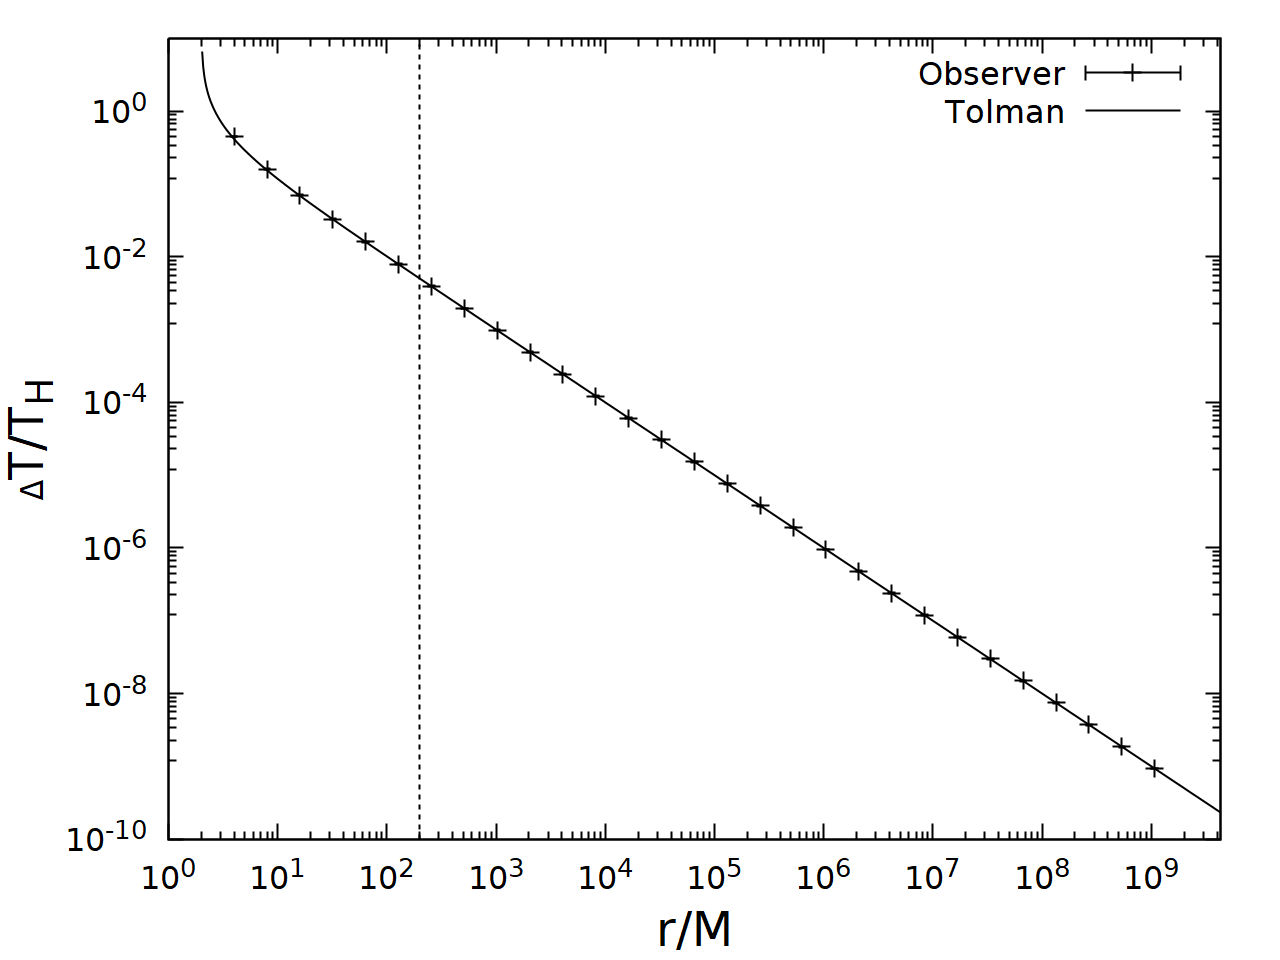
\includegraphics[width=\textwidth]{cpp/final/stat.png}
    \caption{Relative temperature shift}
  \end{subfigure}%
  \begin{subfigure}[h]{0.5\textwidth}
    \centering
    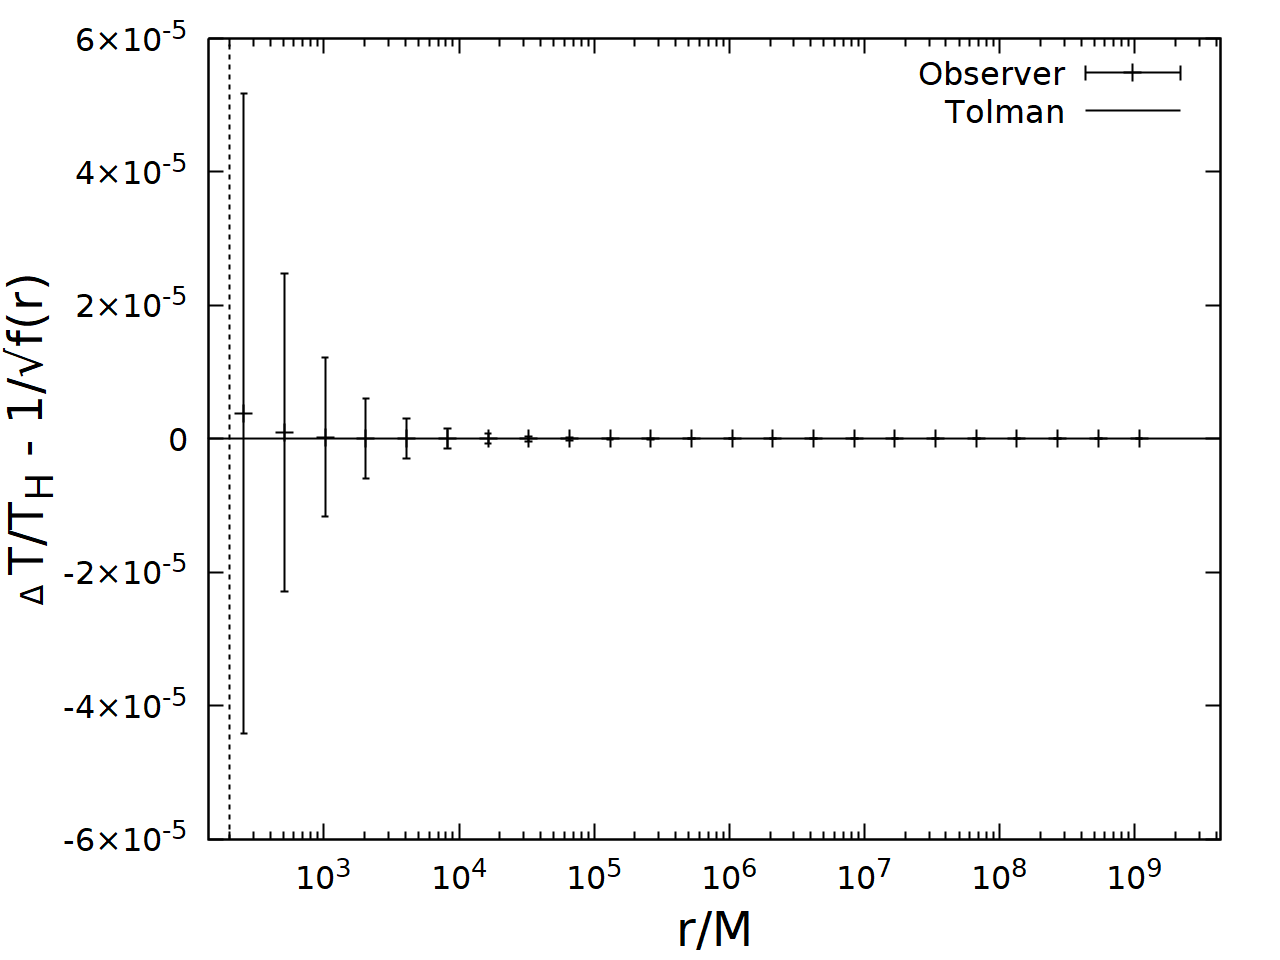
\includegraphics[width=\textwidth]{cpp/final/stat_tolman.png}
    \caption{Difference to Tolman relation}
  \end{subfigure}
  \caption[Static observer]{Static observer -- The relative temperature fits with Tolman-relation as shown in a). In b) the Tolman relation was subtracted. It matches with the Tolman relation within the numerical errors. Below the dotted line at \(r = 200M\) the approximation is not suitable.}
  \label{fig:bh_stat}
\end{figure}
 
\subsection{Circular observer}
\subsubsection{Before the collapse}
By Lemma \ref{lemma:killing} we know that a circular observer should see some excitations. Using our approximate form we can now calculate what he will actually measure. A circular observer is given by \(t = a\tau\), \(\varphi = B\tau\), \(r = \mathrm{const.}\), \(\theta = \frac{\pi}{2}\)\footnote{Since the spacetime is spherically symmetric we can choose a coordinate system such that \(\theta = \frac{\pi}{2}\) and \(B>0\)}. The geodesic equation and \(\dot{\vb{x}}^2 = -1\) give constrains on the constants (see for example \cite{carroll})
\begin{align}
A^2 &= \frac{r}{r-3M}\\
B^2 &= \frac{1}{r^2}\frac{M}{r-3M}
\end{align}

The Wightman function evaluated on the curve is 
\begin{align}
D^+(\vb{x}(\tau), \vb{x}(\tau')) &= -\frac{1}{4\pi^2f(r)} \frac{1}{(A(\tau-\tau')-i\varepsilon)^2 - 2r_*^2 (1 - \cos{B(\tau-\tau')})}
\end{align}

We see that \(D^+\) only depends on \(\tau - \tau'\). So we can use the simplified formular \eqref{equ:qft_detector_final}. For this we need to find the poles in the lower half of \(D^+(\vb{x}(\tau),0)\) which means finding the roots of 

\begin{align}
0 &= A^2\tau^2 - 2r_*^2 (1 - \cos{B\tau})\\
0 &= \xi^2 x^2 - 2(1 - \cos{x})
\end{align}
\todo{footnote}
where \(x = B\tau\) and \(\xi = \frac{A}{Br_*}\). 
Clearly \(\tau = 0\) is a root (which will lie in the upper half\todo{link}). Apart from that we have to differentiate between two cases:
\begin{itemize}
\item \(\xi < 1\): In this case there are another two roots on the real axis. The reason is that for \(\xi < 1\) (which is a very fast circular motion) the trajectory hits the Minkowski-lightcone. But we know that this is not possible in the Schwarzschild-spacetime by the argumentation in section \ref{sec:static_pole}. So we assume that this behaviour is due to our approximation and therefore exclude this case\footnote{Note that \(\xi < 1\) for a geodesic can only happen for \(r \lesssim 1.1 R\ind{S}\) which is definitely not far away from the black hole}.
\item \(\xi > 1\): This case represents slower motions. There are two more (first order) poles at \(\pm i x_0\) of whom one is in the lower half. 
\end{itemize}

The rate is given by eq. \eqref{equ:qft_detector_final}
\begin{align}
\dv{F_E}{\tau} &= \int_{-\infty}^\infty \dd{\tau} e^{-i E \tau} D^+(\vb{x}(\tau), \vb{x}(0))\\
	&= -\frac{1}{4\pi^2f(r)} \int_{-\infty}^\infty \dd{\tau} e^{-i E \tau} \frac{1}{A^2\tau^2 - 2r_*^2 (1 - \cos{B(\tau)})}\\
	&= -\frac{1}{4\pi^2 r_*^2 f(r) B} \int_{-\infty}^\infty \dd{x} e^{-i E x/B} \frac{1}{\xi^2 x^2 - 2 (1 - \cos{x})}\\
	&= \frac{i}{2\pi r_*^2 f(r) B}\mathrm{Res}\qty(e^{-i E x/B} \frac{1}{\xi^2 x^2 - 2 (1 - \cos{x})}, -ix_0)\\
	&= \frac{i}{2\pi r_*^2 f(r) B} e^{-E/B x_0} \lim_{x\to -i x_0} \frac{x + ix_0}{\xi^2 x^2 - 2 (1 - \cos{x})}\\
	&= \frac{1}{2\pi r_*^2 f(r) B} e^{-E/B x_0} \frac{1}{-2\xi^2 x_0 + 2 \sinh{x_0}}
\end{align}

So basically a circular observer sees a exponentially falling energy distribution.
\todo{Erklärung nicht thermisch}

\subsubsection{After the collapse}
An observer on a circular orbit \(t = A \tau\) and \(\varphi = B\tau\) has the following thermal Wightman function:
\begin{align}
D^+_\beta(\vb{x}(\tau),\vb{x}(0)) &= -\frac{1}{4\beta^2 f(r)} \frac{1}{\sinh[2](\frac{\pi}{\beta}\sqrt{A^2\tau^2 - 2 r_*^2 (1-\cos{B\tau})})}
\end{align}

This function is problematic because expanding around zero yields:
\begin{align}
D^+_\beta(\vb{x}(\tau),\vb{x}(0)) &= -\frac{1}{4\pi^2 \tau^2} \frac{1}{f(r) A^2 - f(r)r_*^2 B^2} + \order*{\tau^0}\neq -\frac{1}{4\pi^2 \tau^2} + \order*{\tau^0}
\end{align}

Unfortunately the \(\tau^{-2}\) term has a different prefactor since we are only given \(\dot{\vb{x}}^2 = -f(r) A^2 + r^2 B^2 = -1\). However we know by \ref{sec:static_observers_thermal} that for every non approximate Wightman function on a trajectory this prefactor looks like \(-1/4\pi^2\). So this deviation is due to our approximation which is therefore only applicable if \(r^2 \approx f(r)r_*^2\). For \(r > 200 M\) the deviation is smaller than \(10 \%\). We will ignore smaller values of \(r\) for the interpretation of the results. \todo{plot}

The main problem with the different prefactor is that the difference with another thermal Wightman function will remain divergent at \(\tau = 0\)\footnote{This difference must not be singular since we would like to integrate it numerically, see eq. \eqref{equ:app_num_formula}}. We can deal with this problem by replacing \(r_*^2\) by \(r^2/f(r)\) in the Wightman function
\begin{align}
D^+_\beta(\vb{x}(\tau),\vb{x}(0)) &= -\frac{1}{4\beta^2 f(r)} \frac{1}{\sinh[2](\frac{\pi}{\beta}\sqrt{A^2\tau^2 - 2 \frac{r^2}{f(r)} (1-\cos{B\tau})})}
\end{align}

This is possible because the approximation is only valid when the difference is neglectable. Now we can determine the temperature shift according to section \ref{sec:app_num}. The result is given in fig. \ref{fig:bh_circ}. One can see as long as our approximation is suitable (above the dotted line) the result fits to the Tolman relation. Again the difference between both lies inside the numerical errors.

\begin{figure}[h]
  \centering
  \begin{subfigure}[h]{0.5\textwidth}
    \centering
    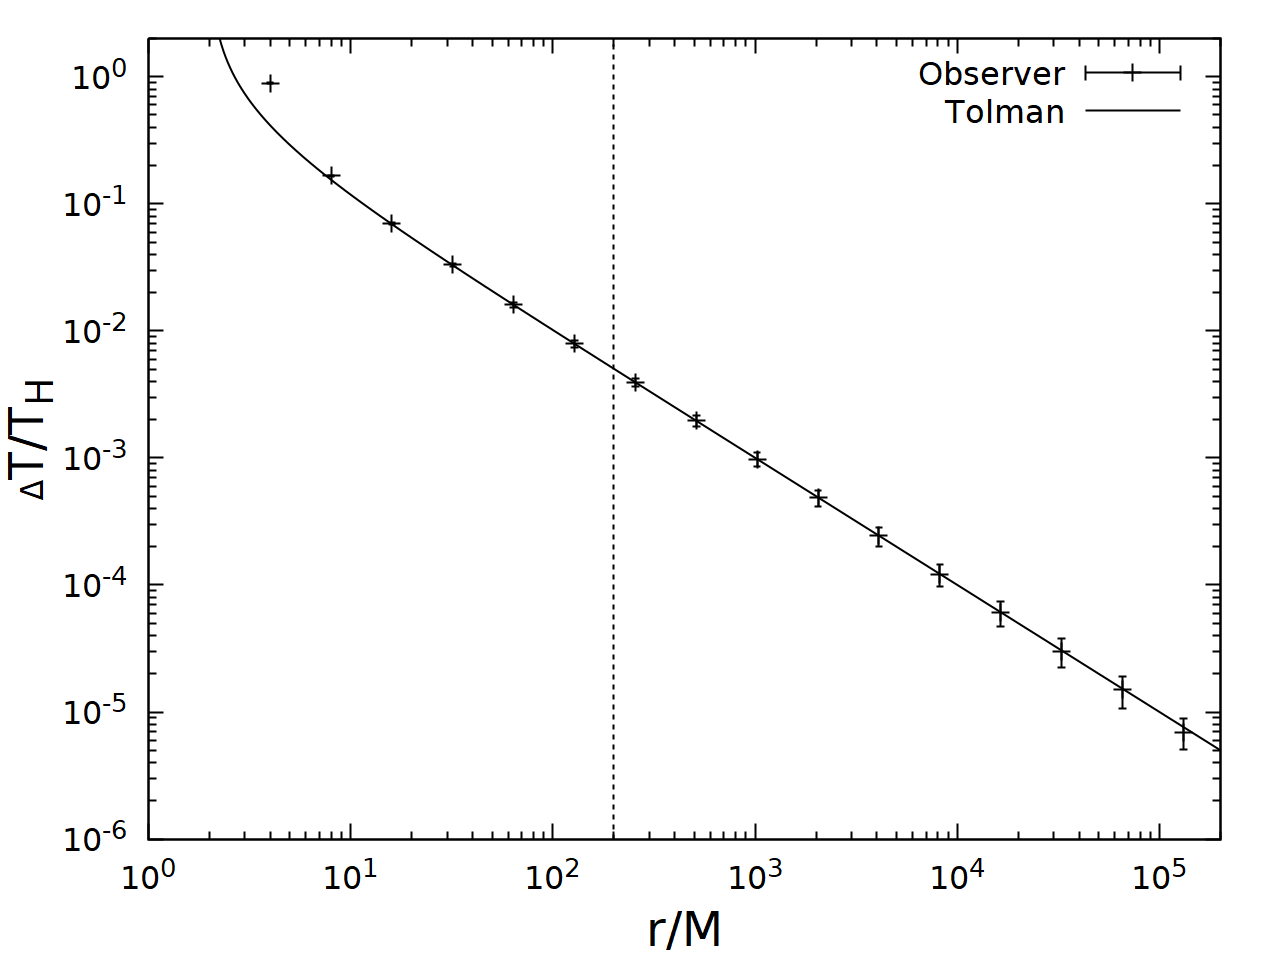
\includegraphics[width=\textwidth]{cpp/final/circ.png}
    \caption{Relative temperature shift}
  \end{subfigure}%
  \begin{subfigure}[h]{0.5\textwidth}
    \centering
    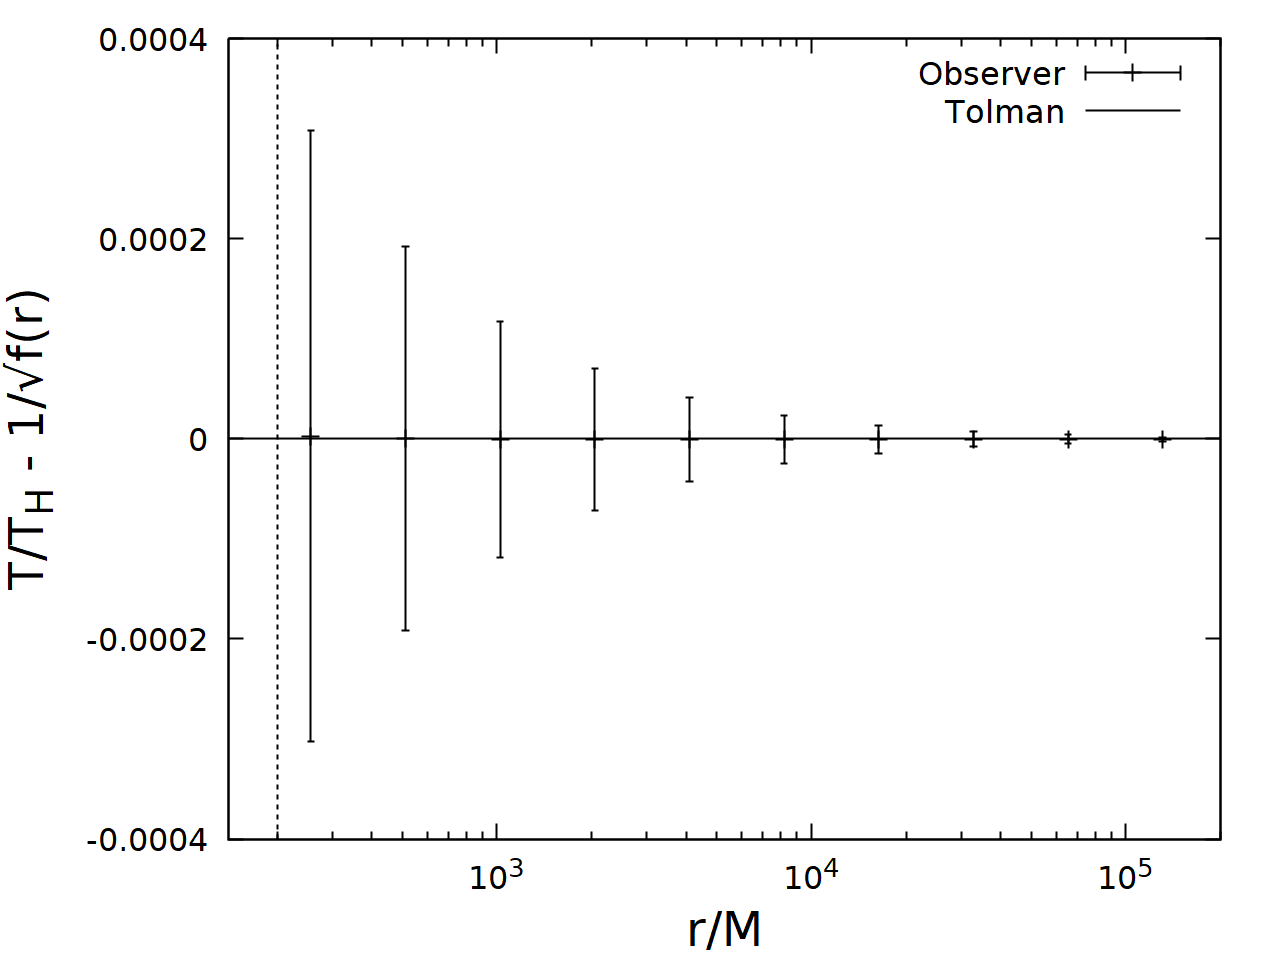
\includegraphics[width=\textwidth]{cpp/final/circ_tolman.png}
    \caption{Difference to Tolman relation}
  \end{subfigure}
  \caption[Circular observer]{Circular observer -- The relative temperature fits with Tolman-relation as shown in a). In b) the Tolman relation was subtracted. It matches with the Tolman relation within the numerical errors. Below the dotted line at \(r = 200M\) the approximation is not suitable.}
  \label{fig:bh_circ}
\end{figure} 

\subsection{Radial observer after the collapse}

We will restrict ourselves to the case of a freely falling observer that is dropped at infinity with zero velocity. This means \(E = f(r) \dot{t} = 1\). The geodesic equation and \(\dot{\vb{x}}^2 = -1\) result in the following trajectory \cite{weinstein}:
\begin{align}
r(\tau) &= \qty(-\frac{3}{2}\sqrt{2M} \qty(\tau - \tau_0))^\frac{2}{3}\\
t(\tau) &= \tau - \tau_0 - 3\tau_0 \qty(\frac{1}{x(\tau)} + \frac{1}{2}\ln \frac{x(\tau)-1}{x(\tau)+1})
\end{align}   

where \(x(\tau) = -\dot{r} = \qty(1-\frac{\tau}{\tau_0})^{-\frac{1}{3}}\) and \(\tau_0 = \frac{4M}{3}\)\footnote{\(\tau_0\) is chosen such that at \(\tau = 0\) the observer hits the event horizon.}. This is inserted in the thermal Wightman function \eqref{equ:bh_wightman_thermal} and the measured temperature is determined (see fig. \ref{fig:bh_rad}).

\begin{figure}[h]
  \centering
  \begin{subfigure}[h]{0.5\textwidth}
    \centering
    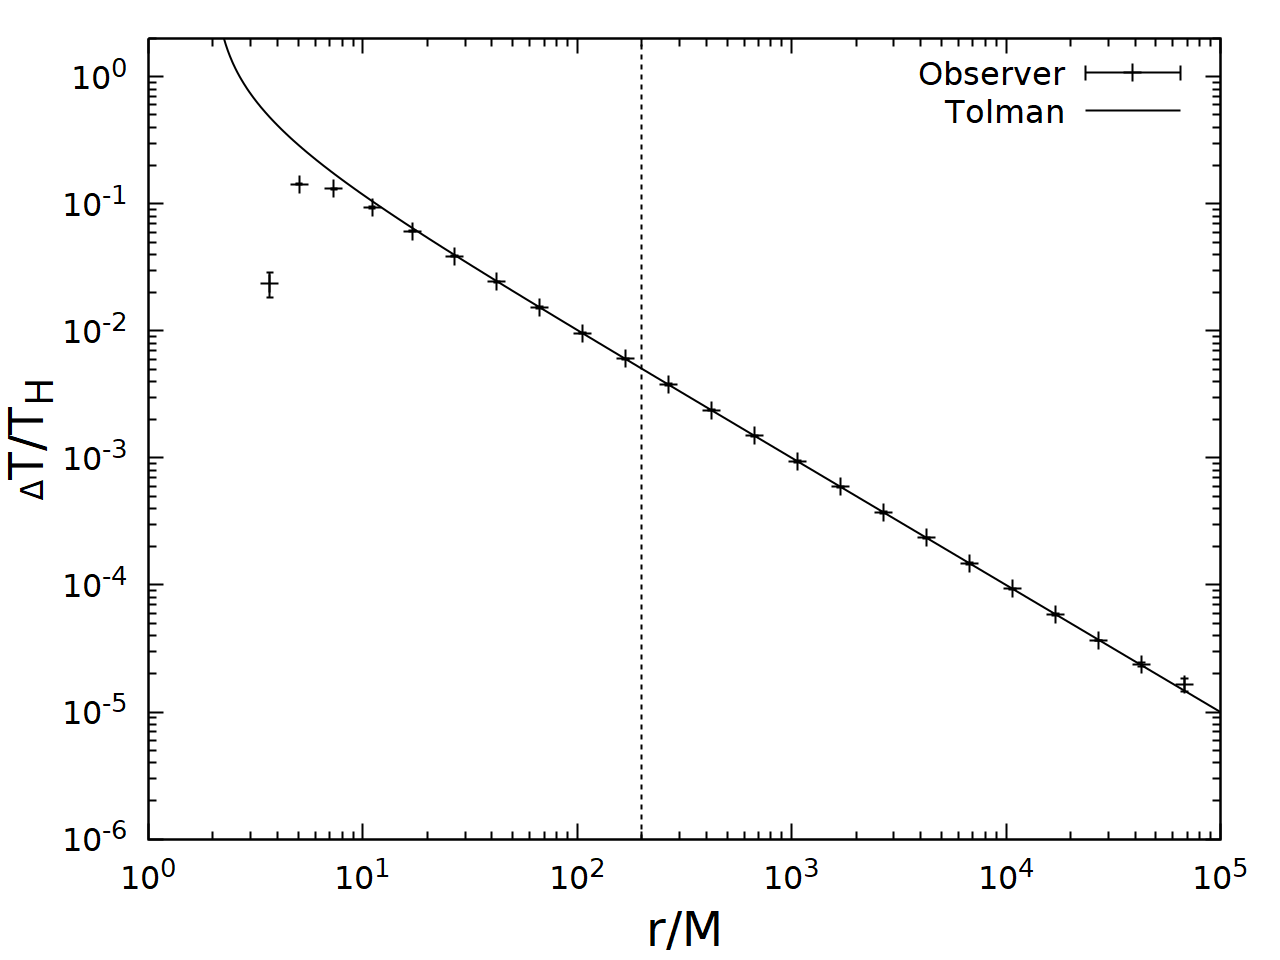
\includegraphics[width=\textwidth]{cpp/final/rad.png}
    \caption{Relative temperature shift}
  \end{subfigure}%
  \begin{subfigure}[h]{0.5\textwidth}
    \centering
    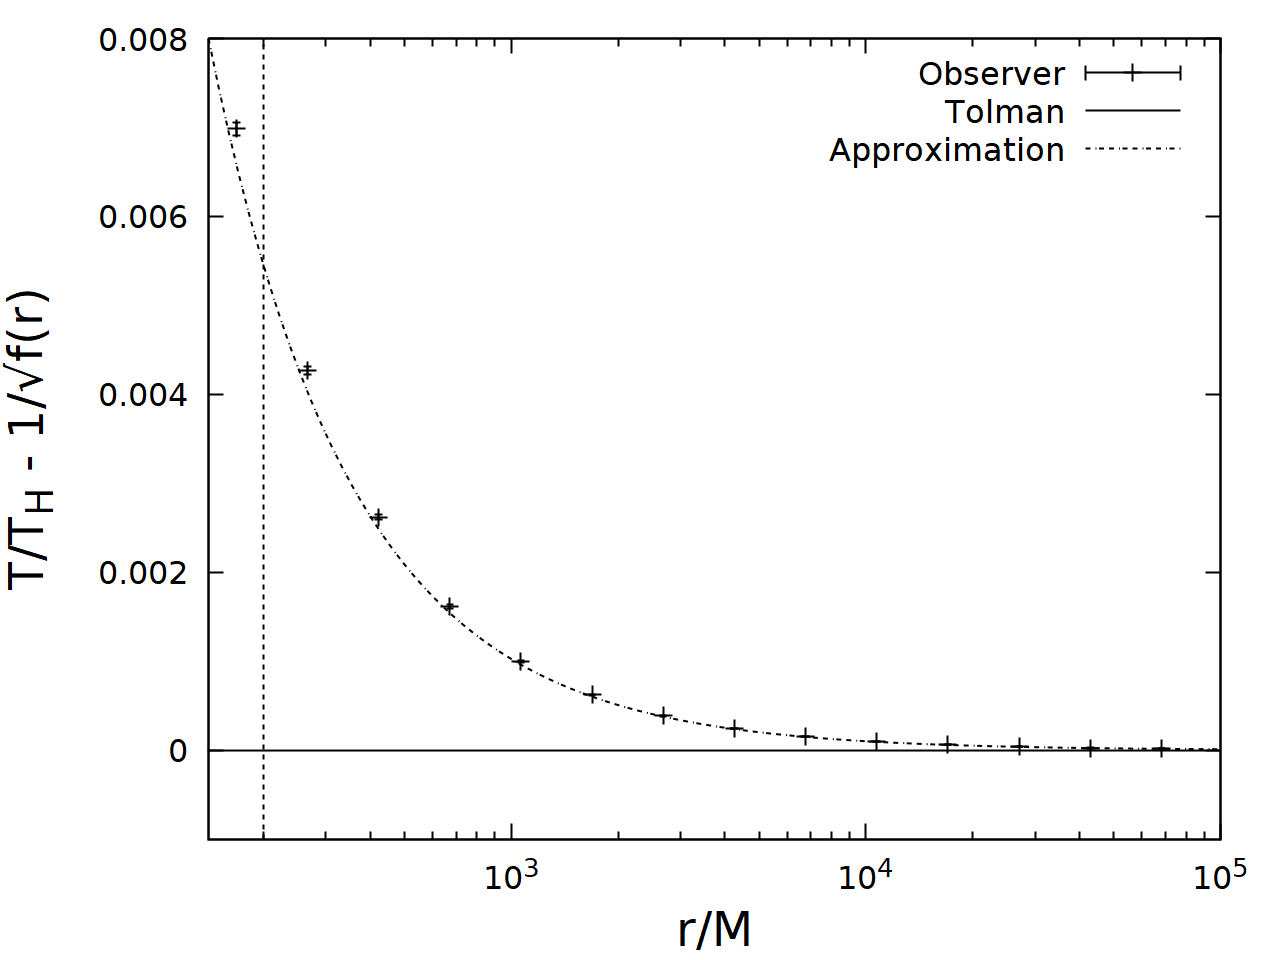
\includegraphics[width=\textwidth]{cpp/final/rad_tolman_error.png}
    \caption{Difference to Tolman relation}
  \end{subfigure}
  \caption[Radial infalling observer]{Radial infalling observer -- The relative temperature fits with Tolman-relation as shown in a). In b) the Tolman relation was subtracted. The difference is outside of the numerical errors even for radii \(r > 200 M\) (dotted vertical line). However the difference has the same order of magnitude of the estimated error caused by approximating the Wightman function (dotted curve).}
  \label{fig:bh_rad}
\end{figure}

The result again fits with the Tolman relation. After subtracting the Tolman relation we find a difference much larger than the numerical errors. Note that the error bars only depict the numerical error, not the error done by approximating the Wightman function. In the last section we found that we can only use our Wightman function when \(\frac{r_*^2}{r^2} f(r) \approx 1\). We need to estimate the order of magnitude of the error caused by this approximation in order to show whether or not the difference in fig. \ref{fig:bh_rad} b) is a significant deviation from the Tolman relation\todo{Fehler berechnen?}. We can give a (rough) estimate by applying the relative error done by the approximation on the Tolman relation, i.e. \(\frac{r_*^2}{r^2} f(r) \cdot \qty(\frac{1}{\sqrt{f(r)}} - 1)\). This is given as a dotted curve in fig. \ref{fig:bh_rad} b). The calculated temperature deviation has about the same order of magnitude. This means that the difference could be completely due to our approximation. We will therefore be conservative and conclude that up to the errors of our method there is no temperature shift for an infalling observer.         